\section{Sweet.JS macro system?}

Sweet.JS~\cite{bib6} is a hygienic macro compiler for JavaScript that takes JavaScript macros and produces normal JavaScript code which one can run in a browser or using a standalone interpreter like Node.JS. The idea is that you define a macro with a name and a list of patterns. Whenever a macro is invoked, the code is matched and expanded at  compile time.

Sweet.JS provides two ways to define a macro: 1) simple pattern based \textit{rule} macros that work by matching a syntax pattern and generating the new pattern based on the template, 2) the more powerful procedural \textit{case} macros allow you to manipulate syntax. The following example shows a rule based macro definition and usage:

\begin{lstlisting}[frame=single]
macro define {
   	 rule { $x } => {
   		    var $x
   	 }
   	 rule { $x = $expr } => {
   	     var $x = $expr
    	}
}
define y;
define y = 5;
\end{lstlisting}

Above code will expand to
\begin{lstlisting}[frame=single]
	var y;
	var y = 5;
\end{lstlisting}


\begin{lstlisting}[frame=single]
SyntaxParameter(<parameter>,<Mapped to>,
<Scope/Macro Name>,<Macro definition>)
\end{lstlisting}

\newpage
\\texttt{parameter} an identifier that is defined as a syntax parameter in the macro definition, \\texttt{Mapped to} is the macro input variable that will be mapped to \\texttt{parameter}, \\texttt{Scope} define the context of the macro definition.

An example of its usage is shown below:



\begin{figure}[htb]
\centering
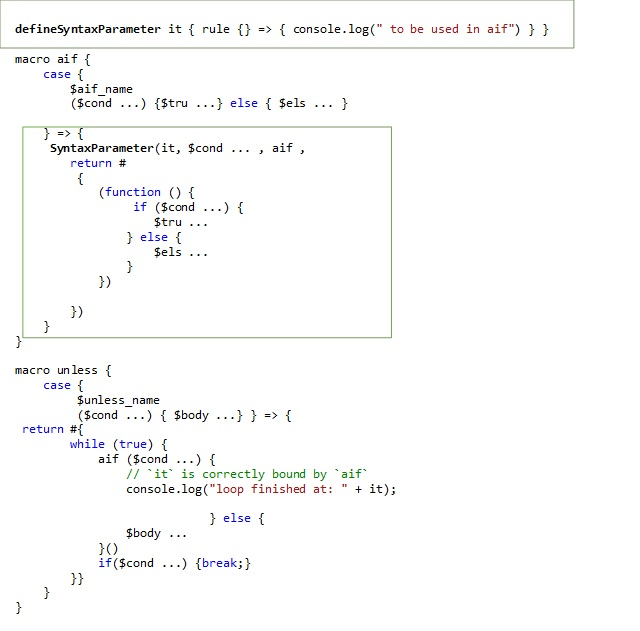
\includegraphics[width=1.0\textwidth]{images/Appraoch1.jpg}
\caption{Approach 1.} 
\label{fig:AST1}

\end{figure}

\begin{figure}[htb]
\centering
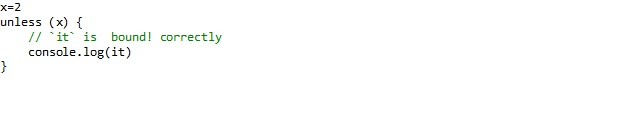
\includegraphics[width=1.0\textwidth]{images/Appraoch2.jpg}
\caption{Calling unless macro} 
\label{fig:AST2}

\end{figure}

The expanded code looks like:

\begin{figure}[htb]
\centering
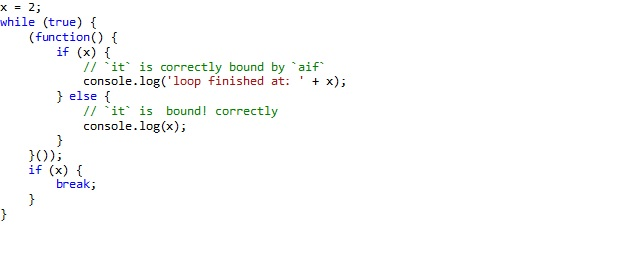
\includegraphics[width=1.0\textwidth]{images/Appraoch3.jpg}
\caption{ it identifier is correctly bounded to \$cond.. Of an anaphoric-if} 
\label{fig:AST3}

\end{figure}

As the example in Figure 10 shows, \\texttt{`it'} is correctly bounded to \$cond.. as desired, However this approach has certain disadvantages, since this won`t allow users to define macros named \\texttt{``SyntaxParameter''} 

At the moment in Sweet.JS the only way to create a syntax transformer is by defining a macro. A macro is really just a function that takes syntax and returns syntax (thus a syntax transformer). To fix this we first need to implement some primitive function that help us to create and manipulate the arbitrary compile time syntax transformation. Macros are compile time syntax transformation , So when the ``expander'' encounters a macro definition it converts the body of the macro into a function and loads it into the compile time environment.